\section{Artifacts, Data Structures, and Other Formalizations}
\label{chap:artifacts}
The assessment processes of critical system development produce important artifacts that are used together for certification of the system, but those of importance to this thesis are \textit{Fault Trees} and associated sets called \textit{Minimal Cut Sets}. For this reason, more information is provided in this section on these artifacts.

\subsection{Fault Trees and Minimal Cut Sets}
The use of fault trees are common in many safety assessment processes and the ability to generate the cut sets needed for the construction of the fault tree is a useful part of any safety analysis tool. The fault tree is a safety artifact commonly referenced in requirement protocol documents such as ARP4761, ARP4754, and AIR6110~\cite{SAE:ARP4761,SAE:ARP4754A,AIR6110}.

A Fault Tree (FT) is a directed acyclic graph whose leaves model component failures and whose gates model failure propagation~\cite{0f356f05e72f43018211b36f97c8854a}. The system failure under examination is the root of the tree and is called the Top Level Event (TLE). The node types in a fault tree are \textit{events} and \textit{gates}. An event is an occurrence within the system, typically the failure of a subsystem down to an individual component. Events can be grouped into \textit{basic events} which occur independently, and \textit{intermediate events} which occur dependently and are caused by one or more other events~\cite{historyFTA}.  These events model the failure of the system (or subsystem) under consideration. The gates represent how failures propagate through the system and how failures in subsystems can cause system wide failures. The two most common logic symbols used in an FT are the Boolean logic AND-gates and OR-gates. An AND-gate is used when the undesired top level event can only occur when all the lower conditions are true. The OR-gate is used when the undesired event can occur if any one or more of the next lower conditions is true. This is not a comprehensive list of gate types; others include voting, inhibit, or negation gates~\cite{0f356f05e72f43018211b36f97c8854a}.
\begin{figure}[h]
\begin{center}
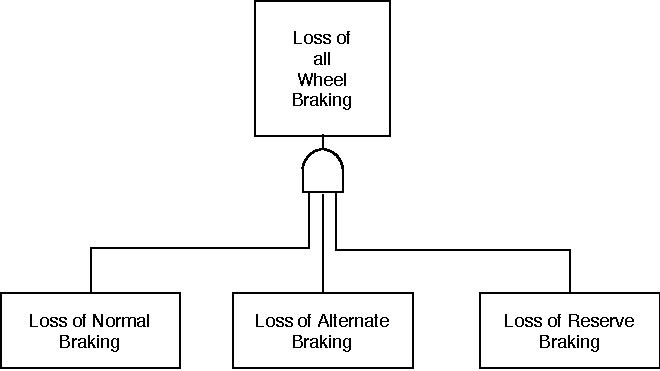
\includegraphics[width=8cm]{images/introFT2.pdf}
\caption{A simple fault tree} \label{fig:introFT}
\end{center}
\end{figure}

Figure~\ref{fig:introFT} shows a simple example of a fault tree based on SAE ARP4761~\cite{SAE:ARP4761}. In this example, the top level event corresponds to an aircraft losing all wheel braking. In order for this event to occur, all of the basic events must occur. This is seen through the use of the AND gate below the top level event. The gates in the fault tree describe how failures propagate through the system. Each gate has one output and one or more inputs. In Figure~\ref{fig:introFT}, the AND gate has three inputs and one output. The leaves of the tree represent the basic events of the system. %and 
In the case of this fault tree, these three events are also the Minimal Cut Sets (MinCutSets) for this top level event. A MinCutSet is the minimal set of basic events that must occur together in order to cause the TLE to occur. Generating and analyzing these MinCutSets is central to FTA and has been an active area of interest in the research community since fault trees were first described in Bell Labs in 1961~\cite{historyFTA,0f356f05e72f43018211b36f97c8854a}. 

There are two main types of fault tree analysis that we differentiate here as \textit{qualitative} analysis and \textit{quantitative} analysis. In qualitative analysis, the structure of the fault tree is considered and the MinCutSets are a way to indicate which combinations of component failures will cause the system to fail. On the other hand, in quantitative analysis, the probability of the TLE is calculated given the probability of occurrence of the basic events~\cite{0f356f05e72f43018211b36f97c8854a}. 

\subsection{Failure Mode and Effects Analysis}
Failure Mode and Effects Analysis (FMEA) was one of the first systematic ways of performing dependability analysis and is used throughout the safety critical industries~\cite{rausand2003system,Bozzano:2011:SDP:1992983.1992988}. FMEA provides a structured way to list possible failures and their consequences systemwide. If probabilities of failures are known, quantitative analysis can be performed to estimate system reliability and to assign critical significance to potential failure modes or system components~\cite{MilStandardFMEA}. Constructing an FMEA table is often the first step in the fault tree construction, for it shows possible component failures and hence basic events~\cite{0f356f05e72f43018211b36f97c8854a}. Usually the FMEA is presented in tabular form (FMEA Table) and as seen in Figure~\ref{fig:} \danielle{make figure}, shows the failures, intermediate events, and undesired states of the system (or violated requirements). 

\subsection{Ordered Binary Decision Diagrams}
A Binary Decision Diagram (BDD) is a data structure used to encode Boolean formulae.
\begin{figure}[!htb]
        \center{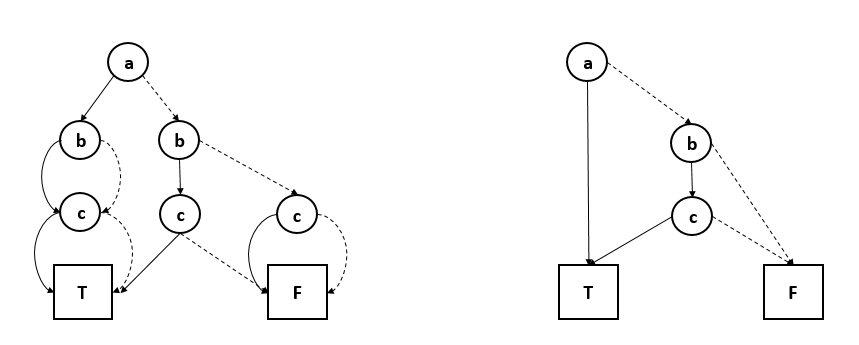
\includegraphics[width=0.8\textwidth] {images/bdd.png}}
        \caption{\label{fig:bdd} Binary Decision Diagrams of the Formula $a \lor (b \land c)$}
\end{figure}
As shown in Figure~\ref{fig:bdd}, it is a rooted, directed, acyclic graph with internal decision nodes and two terminal nodes (\textit{true} and \textit{false}). Each of the decision nodes is labeled with a Boolean variable and has two child nodes, low child and high child. The edge from a node to its low child represents the assignment of \textit{false}, likewise the edge to the high child represents the assignment of \textit{true}. The BDD is called \textit{ordered} if different variables appear in the same order on all paths from the root. Intuitively, following a path from the root to the \textit{true} terminal node represents a valid assignment to the Boolean formula (invalid in the case of ending on the \textit{false} terminal node). 

BDDs are reduced by the removal of isomorphic subgraphs. The BDD shown on the right of Figure~\ref{fig:bdd} is the reduced form of the BDD on the left.

\subsection{Transition Systems}

